\documentclass[10pt,twoside]{article}
%%% PAGE SIZE
\usepackage[paperwidth=5.5in, paperheight=8.5in,margin=0.75in]{geometry}
%%%% HEBREW AND FONT
\usepackage[main=english,bidi=default]{babel}
\babelprovide[import=he]{hebrew}
\babelfont{rm}[Language=English, SmallCapsFeatures = {LetterSpace  =  15,
                            WordSpace  =  { 1.5, 1.5, 1.5},},]{EB Garamond}
\babelfont[hebrew]{rm}[LetterSpace  =  18,
                            WordSpace  =  {1.8, 1.8, 1.8}]{DavidLibre-Regular.ttf}
                            \babelfont[hebrew]{tt}{DavidLibre-Regular.ttf}
                            
\babelfont[hebrew]{sf}{DorianCLMBookItalic.ttf}
\usepackage{calligra}
%%%% NO PAGE NUMBERS
\pagenumbering{gobble}
%%%%% FOR THE PHOTOS
\usepackage{graphicx}
%%%% FOR ADDING NAMES TO THE SERVICE SECTION
\newcommand{\servo}[3]{\textbf{#1}\hfill#2, \textit{#3}\\}
%%%%% INDENTATION
\setlength{\parindent}{1em}

\usepackage{siunitx}
%%%% FOR THE DEMO
\usepackage{lipsum}
%%%%% BORDERS
\usepackage{tikz}
\usepackage{eso-pic}
\usetikzlibrary[calc]
\AddToShipoutPictureBG{%
\begin{tikzpicture}[overlay,remember picture]
%                      V-----------------V
\draw[line width=0.5pt,rounded corners=1cm]
    ($ (current page.north west) + (1.2cm,-1.2cm) $)
    rectangle
    ($ (current page.south east) + (-1.2cm,1.2cm) $);
\end{tikzpicture}
}
\newcommand*{\ClipSep}{0.05cm}%
%%%  SPACING
\usepackage{setspace}

\usepackage{xspace}
\newcommand{\name}{Isaac\xspace}
\begin{document}
\begin{center}
\large\textsc{The Bar Mitzvah of}\\\normalfont\large
\begin{otherlanguage}{hebrew}
הבר מצווה של
\end{otherlanguage}\normalfont
\end{center}

\vspace{0.25in}
\begin{center}
    \Huge\calligra First Middle Last\\\normalfont\huge\sffamily
\begin{otherlanguage}{hebrew}
מושה בן אברהם
\end{otherlanguage}\normalfont

    
\vspace{0.5in}
\begin{tikzpicture}
\node [inner sep=0pt] at (0,0) {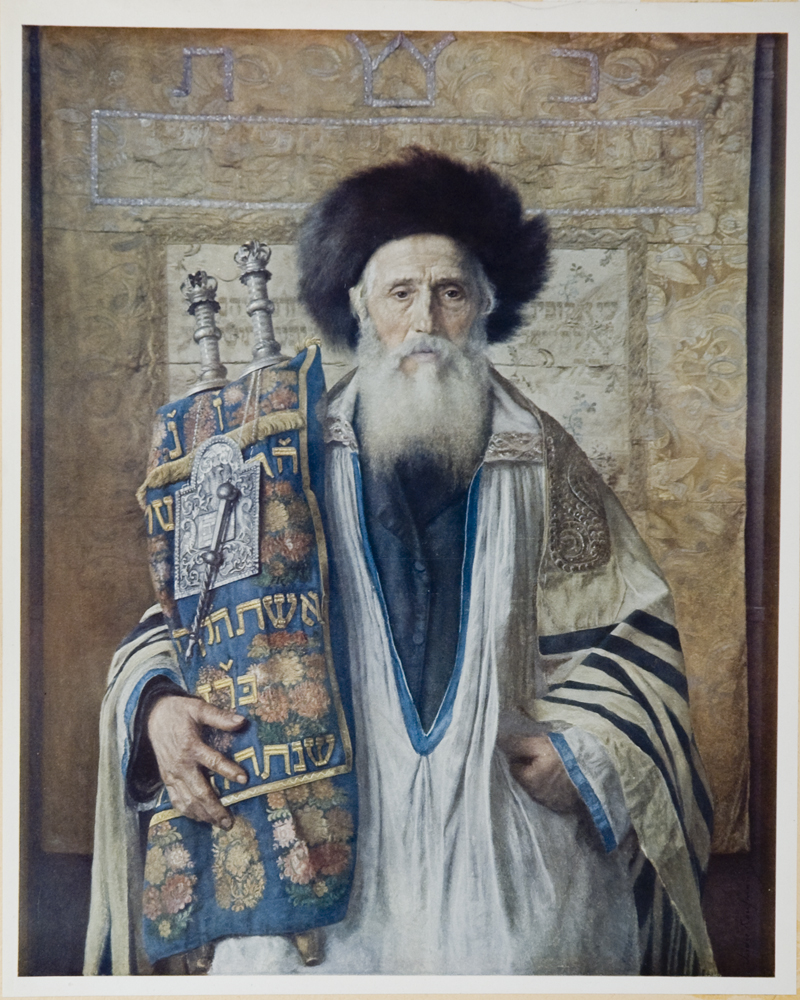
\includegraphics[height=6cm]{rabbi2.jpg}};
\draw [black, rounded corners=\ClipSep, line width=\ClipSep] 
    (current bounding box.north west) -- 
    (current bounding box.north east) --
    (current bounding box.south east) --
    (current bounding box.south west) -- cycle
    ;
\end{tikzpicture}
\end{center}
\vspace{0.25in}
\begin{center}
\normalfont\large\scshape May 15, 2021\\
\begin{otherlanguage}{hebrew}
ה׳ בסיון תשפ״א\\
\end{otherlanguage}
\vspace{0.25in}
Congregation Beth Israel\\
\foreignlanguage{hebrew}{קהילת בית ישראל\scshape}

Town, Place
\end{center}

\clearpage

\begin{center}
\normalfont\calligra\large Shabbat Shalom\end{center}
\lipsum[1]


L'shalom,

\textit{The Stein Family}


 




\begin{center}
\large\calligra About the Service\end{center}

\lipsum[1-2]



\clearpage
\begin{center}
   \large\calligra Bar Mitzvah of Isaac Stein\\\normalfont\normalsize\vspace{0.25in} 
   \servo{Clergy}{Yehuda Rabinstein}{Senior Rabbi}
 \servo{\phantom}{Moishe Hazanowitz}{Cantor}
\servo{\phantom}{Aron Rabinovich}{Junior Rabbi}

\end{center}

\setlength{\parindent}{0em}
\doublespacing
\servo{Presentation of the Tallit}{Name \& Name Stein}{Parents}
\servo{Opening \& Closing of the Ark}{Name Stein}{Brother}\servo{Passing of the Torah}{Name \& Name Stein}{Parents}
\servo{1\textsuperscript{st} Aliyah}{Name \& Name Stein}{Brothers}
\servo{2\textsuperscript{nd} Aliyah}{Name \& Name Stein}{Uncles}
\servo{3\textsuperscript{rd} Aliyah}{Name \& Name Stein}{Grandparents}
\servo{4\textsuperscript{th} Aliyah}{Name \& Name Stein}{Grandparents}
\servo{5\textsuperscript{th} Aliyah}{Name \& Name Stein}{Cousins}
\servo{6\textsuperscript{th} Aliyah}{Name \& Name Stein}{Cousins}
\servo{7\textsuperscript{th} Aliyah}{Name \& Name Stein}{Cousins}
    \servo{8\textsuperscript{th} Aliyah (Maftir)}{Isaac Stein}{Bar Mitzvah}



\begin{center}
   \large\calligra In Memory
   \end{center}
   On this happy day, we take a moment to remember those who cannot be here with us.  May their memories continue to be a blessing.
   
 \servo{\phantom}{Name Stein}{Grandmother}
\servo{\phantom}{Name Stein}{Grandfather}
\servo{\phantom}{Name Stein}{Great-Grandmother}
\servo{\phantom}{Name Stein}{Great-Grandfather}




\clearpage



\vspace{1in}

\begin{center}
    
\includegraphics[height=8.5cm]{etz3.png}
\\\vspace{0.5in}
\calligra\Large``The strength and vitality of a people,\\ like that of a tree,\\ lies in its roots.''
\vspace{1in}

\normalfont\scriptsize Artwork On Front: `Rabbi with Torah' by Isidor Kaufmann, from the Magnes Collection\\. Artwork on Back: `Etz Chaim' by \ttfamily\foreignlanguage{hebrew}{פֿינצטערניש}\normalfont. Both licensed under Creative Commons.\\
Designed in \LaTeX\ by E. Z. Granet.
\end{center}



\end{document}